\documentclass[fr]{article}
%\usepackage{url}
\usepackage[francais]{babel}
\usepackage[utf8]{inputenc}
\usepackage[T1]{fontenc}
\usepackage{fancyvrb}
\usepackage{times}
\usepackage{color}
\usepackage[colorlinks=true,linkcolor=blue,urlcolor=blue,filecolor=blue]{hyperref}
\usepackage{courier}
\usepackage{listings}
\usepackage{float}
\usepackage{enumitem}
\usepackage[table]{xcolor}
\lstset{
  language=C++,
  captionpos=b,
  tabsize=8,
  frame=lines,
  keywordstyle=\color{blue},
  numbers=left,
  numberstyle=\tiny,
  numbersep=5pt,
  breaklines=true,
  showstringspaces=false,
  basicstyle=\small\ttfamily
}

\definecolor{webred}{rgb}{0.5,0,0}
\usepackage{makeidx}
\makeindex
\usepackage{tabularx}
\usepackage{pgf}

\begin{document}
\date{\today}

\title{Rapport sur la réalisation de minishell}
\author{Quentin Deroubaix, Côme David}
\maketitle
%\tableofcontents

\section{Cahier des charges et réalisation}
Le but de mini projet était de se familiariser avec la gestion des
processus et file descriptor dans un environement type Linux. Pour ce
faire, il fallait réaliser un mini-shell qui gérait au moins les pipes
et les redirections.


A l'heure actuelle, notre projet implémente :

\begin{itemize}
\item Une gestion des pipes  
\item redirection >, $\gg$ et <
\item gestion du changement de dossier courant
\item La vérification de la cohérence de la séquence de commandes
  entrée par l'utilisateur
\end{itemize}

\section{Gestion des tableau et des chaines de caractères}
Afin de simplifier l'ecriture du programme, une mini bibliotheque de
gestion des chaines des chaînes de caractères ainsi que des tableaux
de taille dynamique a été crée. Celle ci offre un atout certain afin
de se concentrer sur les problématiques qui sont plus dans le centre
du projet.



\section{Algorithme général}
Nous avons opté pour une gestion récursive de la ligne de commande. 

L'algorithme général est décrit ci dessous : 
\begin{lstlisting}
Lancement du shell 
Si aucun argument fourni dans argv
  Boucleinfinie
  Demander commande
    Si commande valide
      forker() 
      Si pere 
         Attendre son fils
      Si fils 
         Relancer shell avec comme unique argument la commande
  FinBoucle
Si un argument est fourni dans argv
  Compter nombre de pipe dans l'argument
  Si pas de pipe
    Executer la commande
  Si une pipe au moins
     pipe()
     forker()
     Si pere
       Executer la commande la plus a droite
     Si fils
       Relancer le shell avec comme unique argument l'entree utilisateur privee de la derniere commande
%\end{Verbatim}
\end{lstlisting}

En ce qui concerne la gestion des pipes, si l'exécution des commandes se faisait classiquement de gauche à
droite, le premier processus une fois fini signalerai au parent qu'il
pourrait continuer alors que toute la chaîne de pipeline n'est pas
forcement finie. Ici, c'est seulement une fois le dernier processus
fini que le père reçoit un signal comme quoi la séquence est finie.


Visuellement, cela donne quelque chose comme sur la figure \ref{pipe} 
\begin{figure}[!h]
\centering
  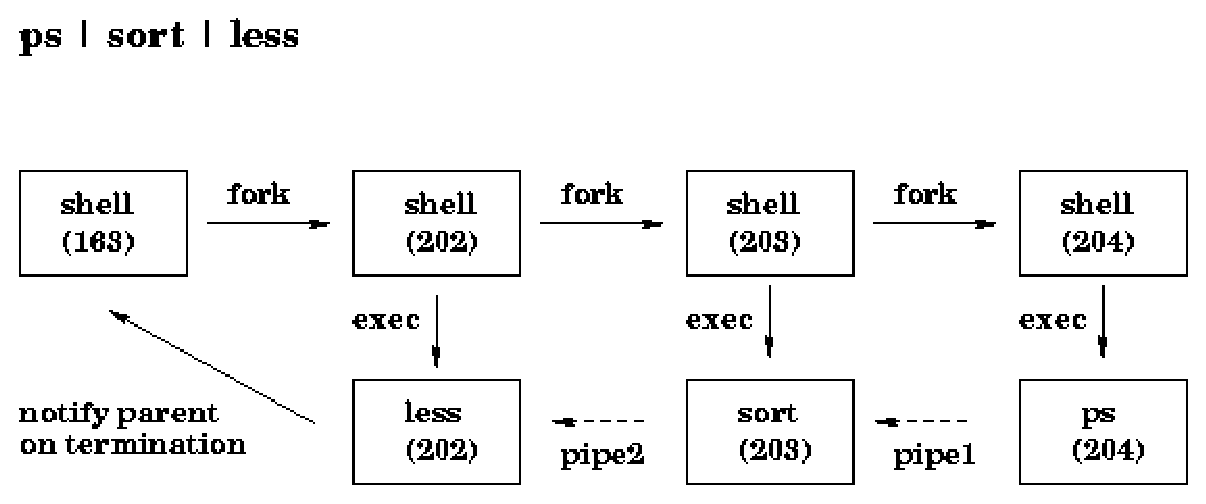
\includegraphics[scale=0.5]{img/pipes}
  \caption{Exemple de gestion des pipes sur la séquence ps | sort | less}
\label{pipe}
\end{figure}

\section{Vérification de la cohérence de l'entrée utilisateur}

Afin de vérifier la cohérence de l'entrée utilisateur, nous avons mis
en place un petit analyseur avec Flex et Bison.

La grammaire est la suivante :
\begin{lstlisting}
  prog: line;
line : cmd_solo | pipe_line |;

cmd_solo: cmd | cmd_in | cmd_out | cmd_inout;

cmd_begin_pipe : cmd | cmd_in;
cmd_end_pipe : cmd | cmd_out;

cmd_in : cmd IN WORD 
;

out_symbol : OUT | OUT_APPEND;
cmd_inout : cmd out_symbol WORD IN WORD
          | cmd IN WORD out_symbol  WORD 
;

cmd_out : cmd out_symbol WORD 
;

cmd : WORD args 
;

arg_word : WORD | QWORD;

args: args arg_word   | {$$="";}
;

pipe_line : cmd_begin_pipe pipe_cmd  ;
pipe_cmd : PIPE cmd pipe_cmd  | PIPE cmd_end_pipe ;
\end{lstlisting}

et le fichier du lexer :

\begin{lstlisting}
  [-\}$\{a-zA-Z0-9_\./]+ { yylval.str = strdup(yytext); return WORD;}

\"([^\\\"]|\\.)*\" {  yylval.str = strdup(yytext); return QWORD;}
\'([^\\\']|\\.)*\' {  yylval.str = strdup(yytext); return QWORD;}

"|" {return PIPE;}
"<" {return IN;}
">" {return OUT;}
">>" {return OUT_APPEND;}

"\n" { return *yytext; } 
\end{lstlisting}
En l'état actuel, il sert juste à accepter ou refuse une séquence de
commande. On pourrait l'utiliser pour remplir des structures afin de 
disposer de la ligne de commande déjà parsée sans avoir à faire appel
à tokenize. Cette évolution n'a pas été réalisée.

\end{document}
